
Neste capítulo será apresentado em detalhes as premissas do problema de classificação visual bem como a metodologia para sua solução, que será particionada nas conforme proposto a seguir. A seção~\ref{sec:Cap3_Dataset} apresenta o conjunto de dados utilizado para o experimento.  A seção~\ref{sec:Cap3_Premissas} apresenta as limitações e condições de contorno do problema. A seção~\ref{sec:Cap3_Proposta} apresenta a proposta de solução para o problema. A seção~\ref{sec:Cap3_Procedimentos} apresenta os procedimentos do experimento para treino e teste do modelo. Dessa forma, a metodologia será seccionada nas seguintes partes:

\begin{itemize}
    \item  Datasets.
    \item  Premissas do problema.
    \item  Proposta de solução.
    \item  Experimento para a solução do problema.

\end{itemize}

% ----------------------------------------------------------

\section{\textit{Conjunto de dados}}\label{sec:Cap3_Dataset}
Foram utilizados dois conjuntos de dados, escolhidos por razões de disponibilidade e representatividade do problema. 

%% Tabelas dos datasets
%- Million A1
%ASGM Ponds Dataset https://zenodo.org/record/6400211
% Planet (URL: https://www.kaggle.com/c/planet-understanding-the-amazon-from-space/data

\subsection{Dataset Amazônia do Espaço}\label{sec:Cap3_Amazon_dataset}

Este conjunto de dados são de imagens coletados dos satélites Planet Flock entre 2016 e 2017. Todas as imagens são da bacia amazônica. Este dataset concerne ao desmatamento e cobrindo condições atmosféricas, coberturas de terreno e fenômenos raros. Cada amostra é um recorde de $256 \times 256$ pixeis RGB, pertencente a uma ou mais das 17 classes distintas e possui resolução espaciais variáveis, por exemplo de $3 m$ por píxel. Este dataset foi publicado pela pela empresa Planet\footnote{https://www.kaggle.com/c/planet-understanding-the-amazon-from-space/data} na plataforma Kaggle, de concursos de aprendizado de máquina.

\begin{figure}[!ht]
    \centering
    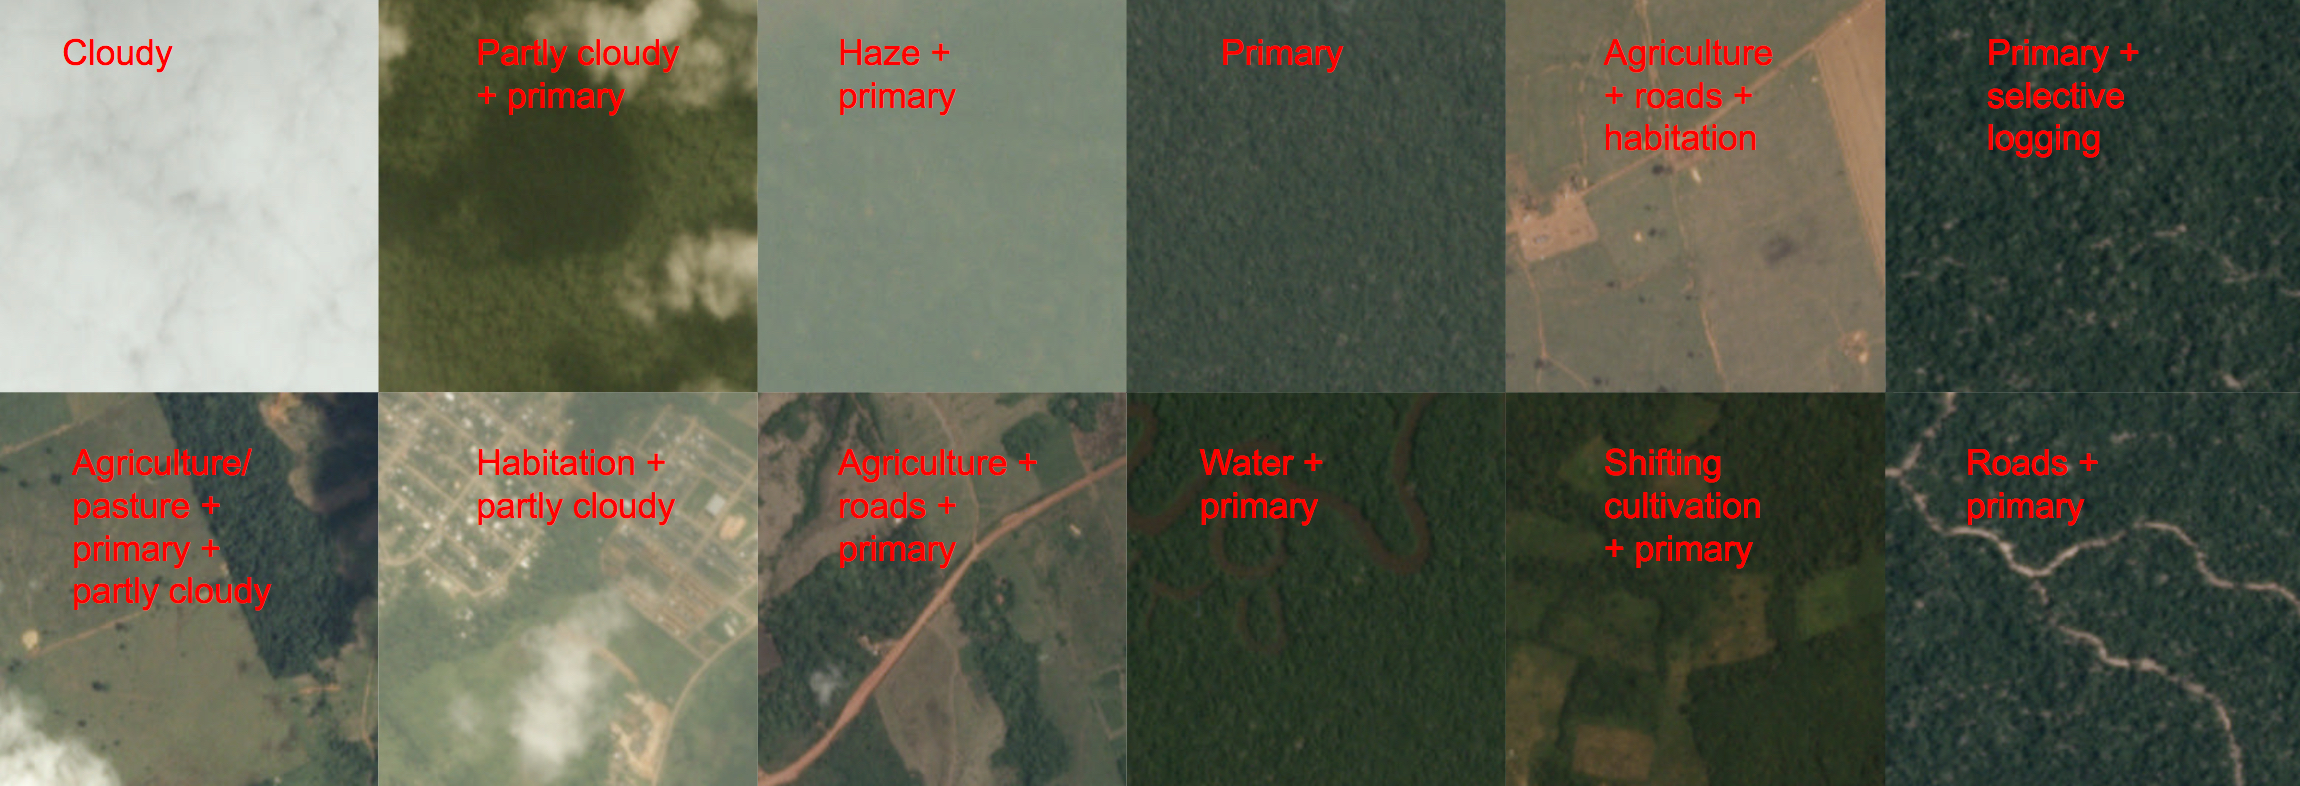
\includegraphics[width=0.9\columnwidth]{
        Imagens/chips.jpg
    }
    \caption{Amostras de classes do dataset Amazônia do Espaço}\label{fig:dataset}
\end{figure}

%We utilize a dataset (URL: https://www.kaggle.com/c/planet-understanding-the-amazon-from-space/data) published in a Kaggle competition (by Planet company), containing coarse-resolution imagery data from satellites with varying spatial resolution characteristics, i.e., the imagery has a ground-sample distance (GSD) of 3.7 m and an orthorectified píxel size of 3 m. The data comes from Planet’s Flock tow satellites in both Sun-synchronous and ISS orbits and was collected in the time interval between January 1, 2016, and February 1, 2017. All of the images are derived from the Amazon basin. Mangrove deforestation in the Amazon forest is an intense phenomenon, and a plethora of factors that contribute to deforestation is observed there. Each entry contains imagery data in RGB plus the infrared band in geo-referenced.tiff format. In our experiment, the images are classified into 14 classes and the labels are broken into three groups: atmospheric conditions, common land cover/land use phenomena, and rare land cover/land use phenomena (see Fig. 3). Here, each entry is assigned to one or more classes.


\subsection{Dataset poças de garimpo}\label{sec:Cap2_amazonia_garimpo}

Este \textit{dataset} foi utilizado em \cite{rs14071746}, mencionado no capitulo anterior. Concerne a tarefa de identificação de mudanças de imagem. Aplicadas a identificação de garimpo artesanal de ouro de pequena escala; Pode ser desafiador de se identificar, dado a variabilidade de condições atmosféricas e baixa resolução. Foram utilizadas imagens de Madre de Dios, região do Peru. Bem como amostras de outros países: Venezuela, Indonésia e Myanmar. 

% (Verificar se esse dataset é utilizável para tarefa de classificação; Resolução parece muito baixa e área muito grande)

% Abstract: Monitoring changes within the land surface and open water bodies is critical for natural resource management, conservation, and environmental policy. While the use of satellite imagery for these purposes is common, fine-scale change detection can be a technical challenge. Difficulties arise from variable atmospheric conditions and the problem of assigning píxels to individual objects. We examined the degree to which two machine learning approaches can better characterize change detection in the context of a current conservation challenge, artisanal small-scale gold mining (ASGM). We obtained Sentinel-2 imagery and consulted with domain experts to construct an open-source labeled land-cover change dataset. The focus of this dataset is the Madre de Dios (MDD) region in Peru, a hotspot of ASGM activity. We also generated datasets of active ASGM areas in other countries (Venezuela, Indonesia, and Myanmar) for out-of-sample testing.


% ----------------------------------------------------------

\section{\textit{Premissas}}\label{sec:Cap3_Premissas}

Temos que o problema de identificação em sensoriamento remoto impõe a dificuldade de alta similaridade extra-classes e divergências intra-classes, da qual surge uma dificuldade de generalização e de viés indutivo para identificação de amostras fora das classes treinadas. Temos ainda que o treinamento de tais modelos envolvem um volume massivo de amostras rotuladas. 


% ----------------------------------------------------------

\section{\textit{Proposta de solução}}\label{sec:Cap3_Proposta}

Como solução para o problema, foi proposta a utilização de um modelo de \textit{transformer visual}  pré-treinado em um conjunto de dados expressivo e realizar o \textit{fine-tune}\footnote{Ajuste fino} para o conjunto de dados de interesse. Dessa forma, obtendo um modelo com boa capacidade de generalização e melhor viés indutivo, assim demandando menor quantidade de amostras para ser treinado.

Para solucionar o problema de generalização e conjunto de dados limitado da região de interesse, propomos a utilização de um modelo pré-treinado explicado em~\ref{sec:Cap2_transfer} um dataset extensivo de imagens aéreas e de satélites, de forma a aproveitar seu extrator de características, como é realizado em~\cite{wang2022empirical}. Assim o modelo será re-treinado (\textit{fine tunning}) para a região de interesse mantendo os pesos das camadas de encoder otimizar apenas a camada MLP fortemente conectadas, assim como a camadas de saídas softmax. 

Dessa forma, a arquitetura proposta é o ViT apresentado em~\cite{wang2022empirical}
composta por camadas hierarquicas de encoders transformers  que funcionam como extratores de características. As camadas seguintes são camadas totalmente conectadas seguidas por uma camada \textit{softmax} que realiza a classificação.
% ----------------------------------------------------------

\section{\textit{Ambiente e ferramentas}}\label{sec:Cap3_Ferramentas}


O Ambiente dos experimentos será em cadernos \textit{Jupyters}, para ser facilmente replicável e ser executável em nuvem, com a possibilidade de alugar recursos computacionais da plataforma em nuvem \textit{Google Colab}. Também será utilizado o \textit{framework PyTorch}, por razões de disponibilidade de métodos e conhecimentos do autor. 

% JupyterLab is the latest web-based interactive development environment for notebooks, code, and data. Its flexible interface allows users to configure and arrange workflows in data science, scientific computing, computational journalism, and machine learning. A modular design invites extensions to expand and enrich functionality. https://jupyter.org

\subsection{\textit{Ambiente}}\label{sec:Cap2_Ambiente}

Foram dispostos 100h de orçamento de recursos computacionais, em uma instância da plataforma com GPU NVidia Tesla T4 de 12 GB de RAM. CPU Intel(R) Xeon(R) CPU @ 2.20GHz, 12 GB de memória. Para o treinamento de redes neurais profundas, aceleradores como placas gráficas podem resultar em ganhos de tempo de até 40x em com paração com treinamentos em CPU, bem como o uso da ram para placa gráfica para realizar \textit{caching}\footnote[1]{Caching é o processo de utilizar um espaço de memória para o armazenamento temporário e de acesso rápido de dados que possuem uma grande probabilidade de serem utilizados novamente} obtendo melhores tempos de acesso durante carregamentos.


\subsection{\textit{Bibliotecas}}\label{sec:Cap2_NumpyPandas}

Para o experimento também contou-se com bibliotecas de calculo numérico e algébrico como o Numpy. Também Pandas para manipulação de dados tabulares. Já a ferramenta SciKitLearn contém diversos módulos para aprendizado estatístico, como funções de métricas, de perdas. Para visualização dos resultados utilizado serão MatplotLib, Plotly e Seaborn.

\subsection{\textit{PyTorch}}\label{sec:Cap2_PyTorch}
Pytorch é um \textit{framework}\footnote{Ferramental} de processamento de tensores e acelerados por GPU\footnote[3]{Unidade de Processamento Gráfico, Trad.:\textit{Graphic Process Unit}} ou TPUs \footnote{Unidade de Processamento de Tensores. Trad. de \textit{Tensor Processing Unit}} para aprendizado de máquina profundo. É código aberto de de front-end em Python, implementado em linguagens C++ e CUDA para otimizações de computações numéricas, matriciais e de difenciação, que são extensivas para esta aplicação.
O projeto é originalmente criado pelo \textit{Facebook Research} e é atualmente amplamente adotado pela academia e mercado em aplicações de aprendizado profundo. Possui muitas implementações das ferramentas mais utilizadas, especificamente aplicadas a \textit{Deep Learning} e visão computacional. Tem ampla adoção devido à intenção de ser um \textit{framework} de fácil uso e alto nível, com muitas abstrações e técnicas já implementadas.

%http://pytorch.org

% ----------------------------------------------------------

\section{\textit{Experimentos}}\label{sec:Cap3_Experimentos}

Para a construção da solução desejada, experimentaremos combinar um modelo pré-treinado com camadas internas, correspondente ao extrator de características e de saída treinadas para a região de interesse.
Consiste em fazer experimentos em uma complexidade crescente, e replicando resultados para garantir corretude. Será simplificado a reprodução para apenas um \textit{dataset}.


Para obter o modelo proposto e de melhor desempenho, inicialmente define-se os seguintes passos de experimentos para construir o modelo final:

\begin{enumerate}
\item   Análise exploratória dos dados, visando a melhor conhecer o problema e amostras. 
\item   Disponibilizar pre-processamento do conjunto de dados e de carregadores de amostras.
\item   Elaborar e treinar um modelo baseline RESNET-18 pré-treinado, fazendo ajuste de hiperparâmetros a fim de obter o melhor score no baseline
\item   Utilizar pesos do dos trabalhos~\ref{sec:Cap2_million} com \textit{checkpoints}\footnote{Captura dos pesos de uma rede a partir de certo ponto do processo de treino} disponibilizados, a fim de replicar a metodologia de fine-tune. 
\item   Realizar o mesmo para o modelo proposto de transformers visuais
\item   Fixar os hiperparâmetros e metodologia de treino para modelos baseline e proposto e treiná-los novamente a fim de realizar comparações
\item   Realizar análise dos resultados de ambos e comparar performance em várias métricas relevantes ao problema
\item   Comparar modelos e com trabalhos base \ref{sec:Cap2_ForestViT} 
\end{enumerate}


    
% ----------------------------------------------------------

\section{\textit{Procedimentos}}\label{sec:Cap3_Procedimentos}

Os procedimentos do experimento principal consiste principalmente nas etapas de configuração do ambiente, pré-processamento do conjunto de dados, análise exploratória, definição do modelo e iterações de treino-validação. Explicadas adiante.

\subsection{\textit{Configuração de Ambiente}}\label{sec:Cap3_ConfigAmbiente}

A plataforma GoogleColab consiste em uma instancia alocada temporariamente com custo por tempo de uso, porém com desconexão por tempo ocioso. Durante o treinamento a interface se torna ociosa e ocorrem desconexões. Para mitigar isto foram criadas funções de gerenciar contexto do experimento, para implementar o armazenamento e carregamento se estatisticas do treinamento a cada epoch.

Os arquivos compactados de são obtido de hospedagem em nuvem e descompactado na instância, seja em disco ou em partição na memória ram. Esta segunda opção permitiu importantes melhorias de tempo de carregamento de batches\footnote[1]{Número de amostras processadas entre atualizações de modelo}. O arquivo contendo os pesos do modelo para criação do modelo são obtidos da mesma forma. Com cada instância é volátil, sendo possível armazenar conteúdos somente no serviço de hospedagem GoogleDrive, os resultados, pesos do modelo e contexto do experimento precisam ser salvos a cada execução, em caso de desconexão.


\subsection{\textit{Análise de dados exploratória}}\label{sec:Cap3_AnaliseDeDadosExploratoria}
Para melhor entendimento das características do conjunto de dados, se faz necessário uma exploração dos dados. Consiste em entender os diferentes tipos de amostras e rótulos, por meio de estatísticas de distribuição de classes e visualizações de agrupamento.


Pela distribuição de classes em \ref{tab:proporcao_classes}, podemos observar que se trata de um dataset com acentuado desbalanço. Contem certos eventos raros como o chamado de Roça de ventos, que consiste de um evento climático gerador de ventos de mais de 160 Km/h que devasta uma vasta área de floresta. Na figura \ref{fig:classes} a seguir podemos visualizar amostras de cada tipo de classe. Cada amostra pode a mais de um tipo de classe.  

\begin{table}[h!]
    \caption{Proporção de Classes do conjunto de dados \textit{Planet}}
    \centering
\begin{tabular}{*{4}{c}}
    \toprule
    Classe                  &            Rótulo &  Amostras      &  Proporção (\%) \\
    \midrule
    Mina Convencional       & conventional mine &        100     &       0,247 \\
    Roça de Ventos          &         blow down &        101     &       0,250 \\
    Queimada                &        slash burn &        209     &       0,516 \\
    Florescimento           &          blooming &        332     &       0,820 \\
    Garimpo                 &    artisinal mine &        339     &       0,837 \\
    Desmatamento Seletivo   & selective logging &        340     &       0,840 \\
    Área Descoberta         &       bare ground &        862     &       2.129 \\
    Nublado                 &            cloudy &       2089     &       5.161 \\
    Névoa                   &              haze &       2697     &       6.663 \\
    Habitação               &        habitation &       3660     &       9.042 \\
    Cultivação              &       cultivation &       4547     &      11.233 \\
    Parcialmente Nublado    &     partly cloudy &       7261     &      17.938 \\
    Águas                   &             water &       7411     &      18.308 \\
    Estrada                 &              road &       8071     &      19.939 \\
    Agricultura             &       agriculture &      12315     &      30.423 \\
    Clima Limpo             &             clear &      28431     &      70.236 \\
    Vegetação Primária      &           primary &      37513     &      92.673 \\
    \bottomrule
\end{tabular}
\label{table:proporcao_classes}
\end{table}




\begin{figure}[!ht]
    \centering
    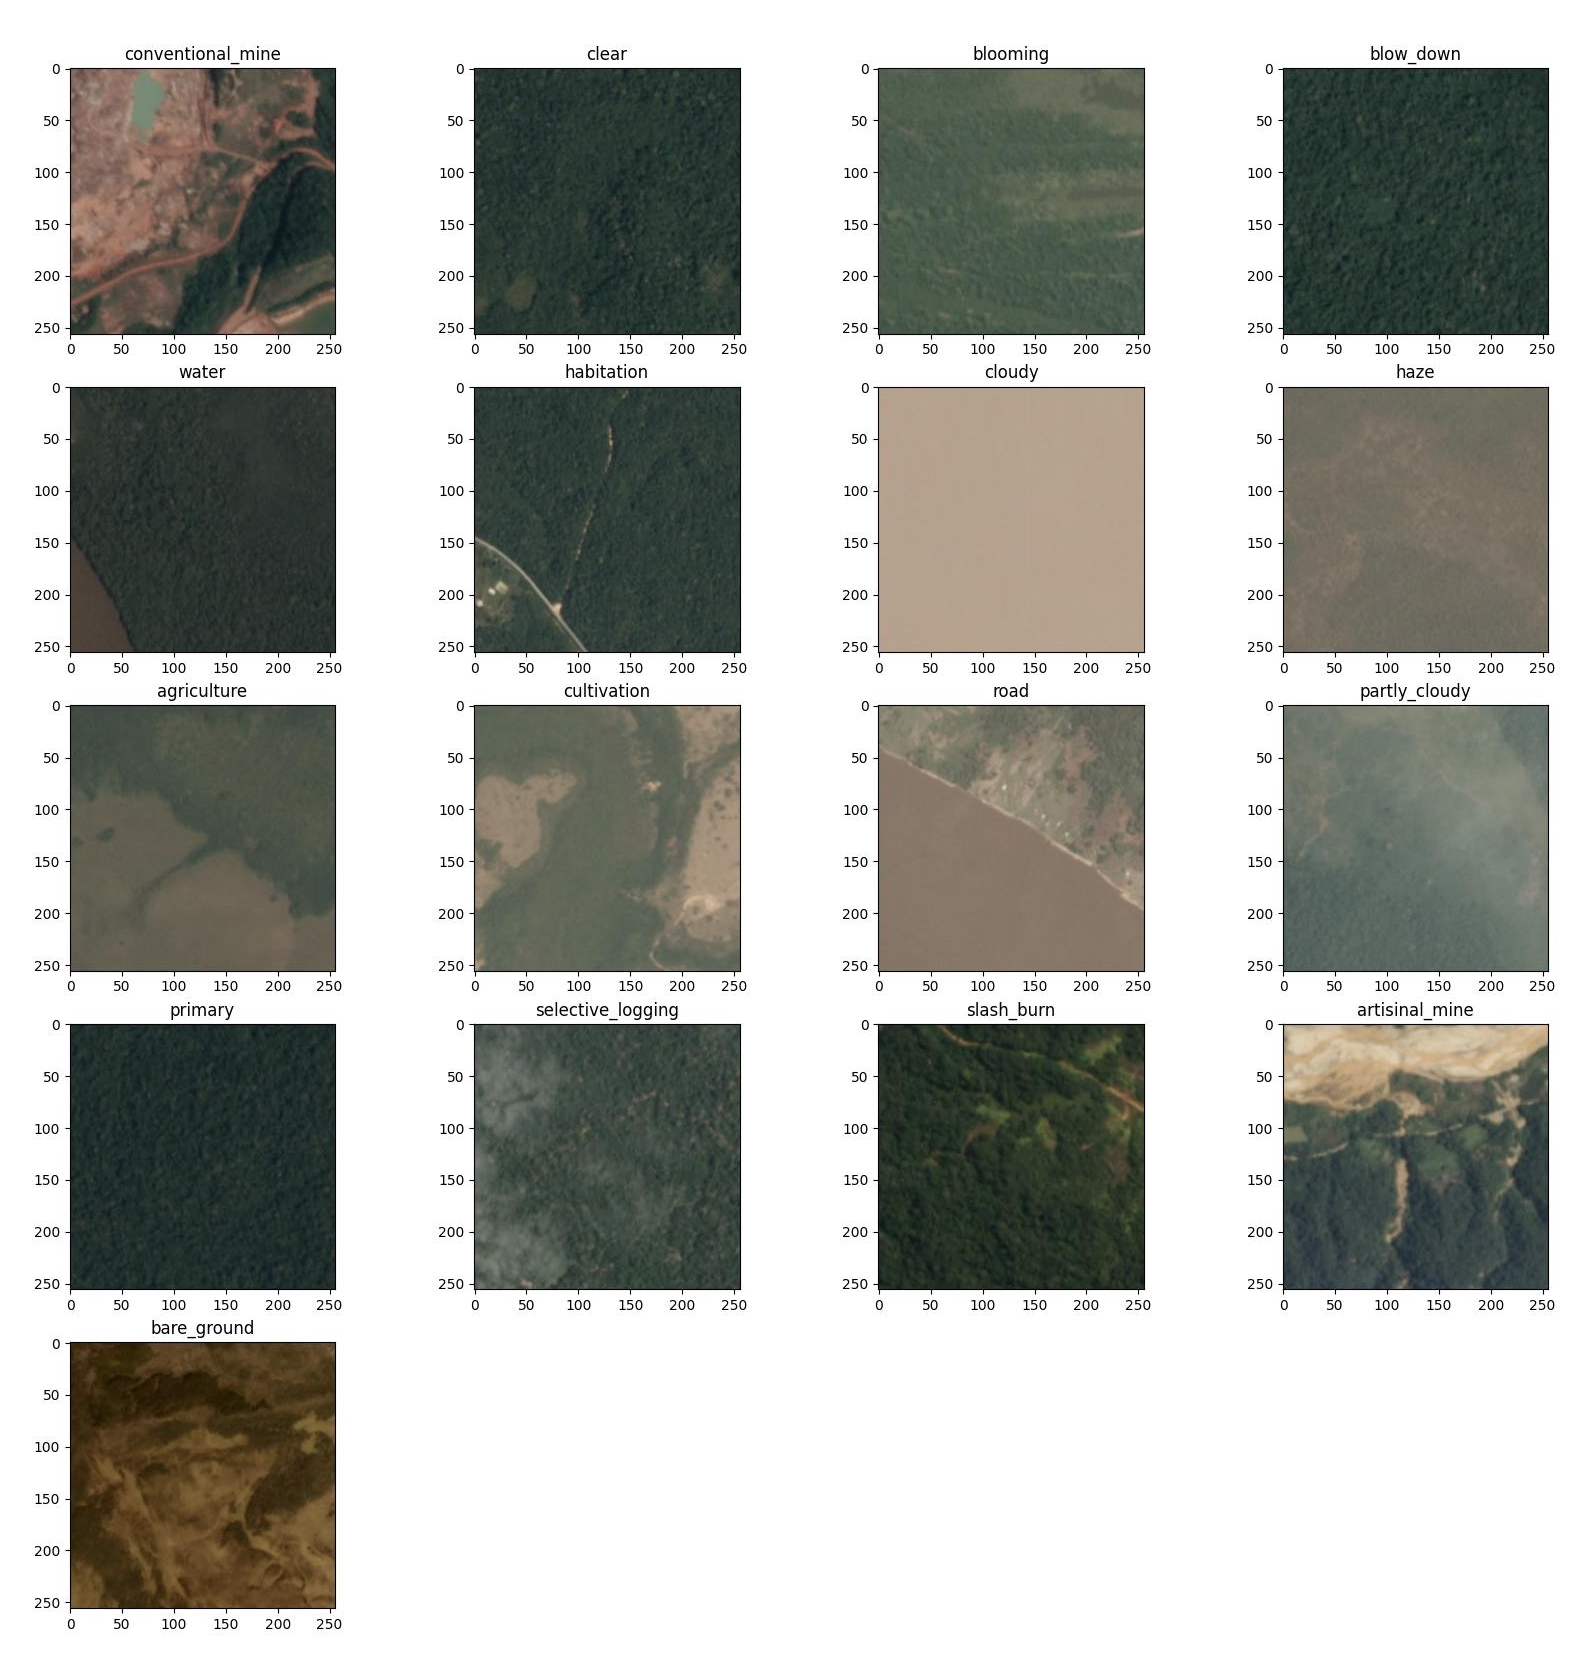
\includegraphics[width=\columnwidth]{Imagens/results/EDA/Class Sampling.jpg}
    \caption{Amostragem de cada classe de rótulo.
    Fonte: Autor}
   \label{fig:classes}
\end{figure}


\begin{figure}[!ht]
    \centering
    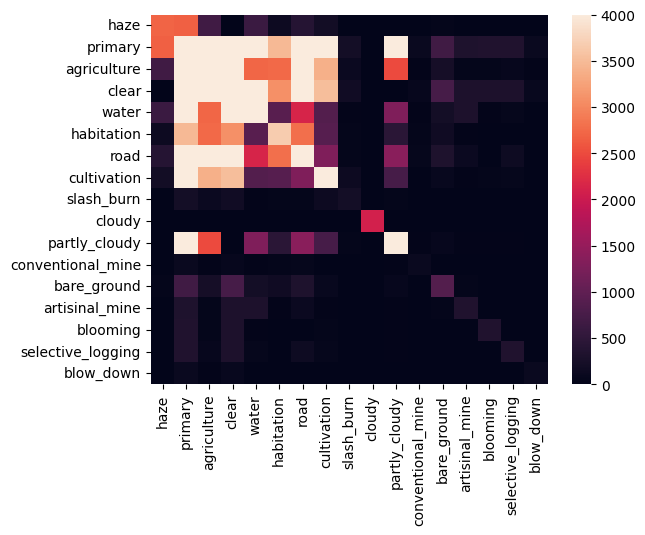
\includegraphics[width=0.5\columnwidth]{Imagens/results/EDA/matriz de coocorrencia.png}
    \caption{Matriz de co-ocorrência.
    Fonte: Autor}
   \label{fig:coocorrencia}
\end{figure}

\begin{figure}[!ht]
    \centering
    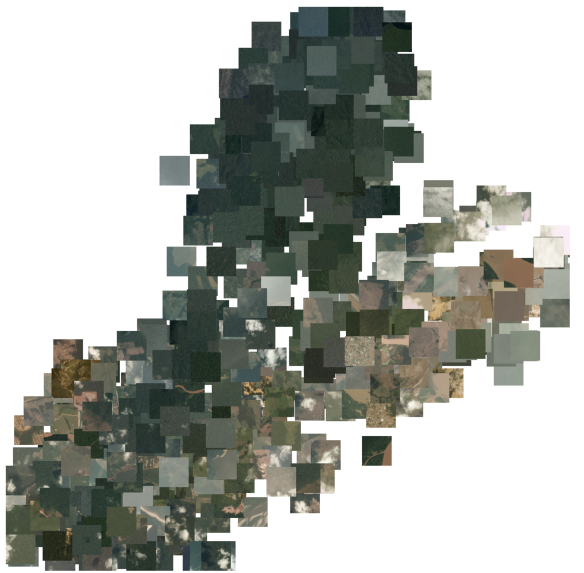
\includegraphics[width=0.9\columnwidth]{Imagens/results/EDA/TSNE.png}
    \caption{Agrupamento de amostras via técnica TSNE.
    Fonte: Autor}
   \label{fig:TSNE}
\end{figure}

A partir da matriz de coocorrência, podemos averiguar sobreposições de classes mais frequentes. É possível constatar que as amostras relacionadas a vegetação primária, agricultura e águas são as predominantes. Quanto ao clima, também há sobreposição de classes. Contudo para as classes raras, são em sua maior parte independentes entre si.

Outra técnica de semelhança entre amostras é o t-SNE\footnote[5]{T-distributed Stochastic Neighor Embedding} que é um método de redução de dimensionalidade para dados de alta dimensionalidade e projeção em espaço de baixa dimensões. Assim é possível realizar agrupamentos de amostras proximas num espaço de representação. Na figura \ref{fig:TSNE} podemos verificar grupos de amostras visualmente próximos que serão desafiadores de realizar uma classificação precisa. FONTE


\subsection{\textit{Pré-processamento}}\label{sec:Cap3_PreProcess}
O pré-processamento consiste em preparar as amostras do conjunto de dados de interesse para treino e validação. Para o conjunto de dados floresta amazônica temos 40000 amostras. Foram separadas em uma divisão de treino-validação na proporção 80\%-20\%. Cada recorte de resolução $256 \times 256$ px.

O pré-processamento em cada amostra é feito em tempo de execução por instâncias de transformação composta de:
\begin{enumerate}
    \item   Carregamento dos canais RGB e descartando o de infravermelho-próximo de cada imagem.
    \item   Redimensionamento usando interpolação linear de $256 \times 256px$ para $224 \times 224px$. Isto se deve ao fato dos modelos já terem sido pré-treinados e configurados para essa dimensão de entrada.
    \item   Conversão da imagem para estrutura de dados numérica de Tensor
    \item   Aplicar espelho vertical ou horizontal, cada um com probabilidade de 25%.
    \item   Normalizar cada canal de cor RGB usando normalização Gaussiana com médias e desvio padrão do dataset ImageNet.
\end{enumerate}


\subsection{\textit{Definição do modelo}}\label{sec:Cap3_Def_modelo}


Para a definição do modelo, é interessante começar com modelos de menor capacidade, e ao longo da sintonização poder trocar por um de maior capacidade. Por isso, para o experimento base primeiro utilizou-se o modelo ResNet-18 e depois de validado utilizou-se o ResNet-50. Da mesma forma, a implementação do modelo Swin disponibilizado pelo autor de menor capacidade é o \textit{Swin-Tiny}, de número de parâmetros e desempenho próximo ao ResNet50 em \textit{benchmarks} no dataset Imagenet-1k.

\begin{table}[h!]
    \caption{Caracteristicas do modelo fornecida pela biblioteca } 
    \centering
\begin{tabular}{*{8}{c}}
    \toprule
    Nome & Pré-Treino & Resolution & Acuracia@1 & Acuracia@5 &  Parâmetros & FLOPs \\
    \midrule
    Swin-T & ImageNet-1K & 224x224 & 81.474 & 95.5 &	28.3M &	4.5G \\
    Resnet50 & ImageNet-1K & 224x224 &	80.858 & 92.9 &	25.5M &	4.1G \\
    % https://pytorch.org/vision/main/models/generated/torchvision.models.swin_t.html
    \bottomrule
\end{tabular}
\label{tab:especificacao_modelos}
\end{table}

\iffalse
MODEL:
  TYPE: swin
  NAME: swin_tiny_patch4_window7_224
  DROP_PATH_RATE: 0,2
  SWIN:
    EMBED_DIM: 96
    DEPTHS: [ 2, 2, 6, 2 ]
    NUM_HEADS: [ 3, 6, 12, 24 ]
    WINDOW_SIZE: 7
    
\fi 


O modelo Swin proposto corresponde a figura \ref{fig:Swin-T-Rsp}. Foi elaborado a partir de uma instanciação de um classificador de mesmo \textit{backbone} da biblioteca de modelos timm. Em seguida foram a camada de saida, chamada de cabaça do transformer, por uma camada completamente conectada, de tamanho de entrada o número de dimensões do espaço de estados e a dimensão de saída o número de atributos/classes.

\begin{figure}[!ht]
    \centering
    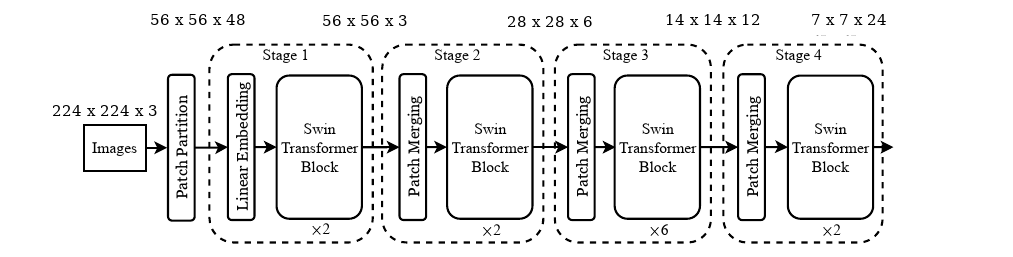
\includegraphics[width=0.9\columnwidth]{Imagens/swin proposto.png}
    \caption{ Arquitetura de modelo proposto.
    Fonte: \cite{liu2022swin}}
   \label{fig:Swin-T-Rsp}
\end{figure}

\begin{figure}[!ht]
    \centering
    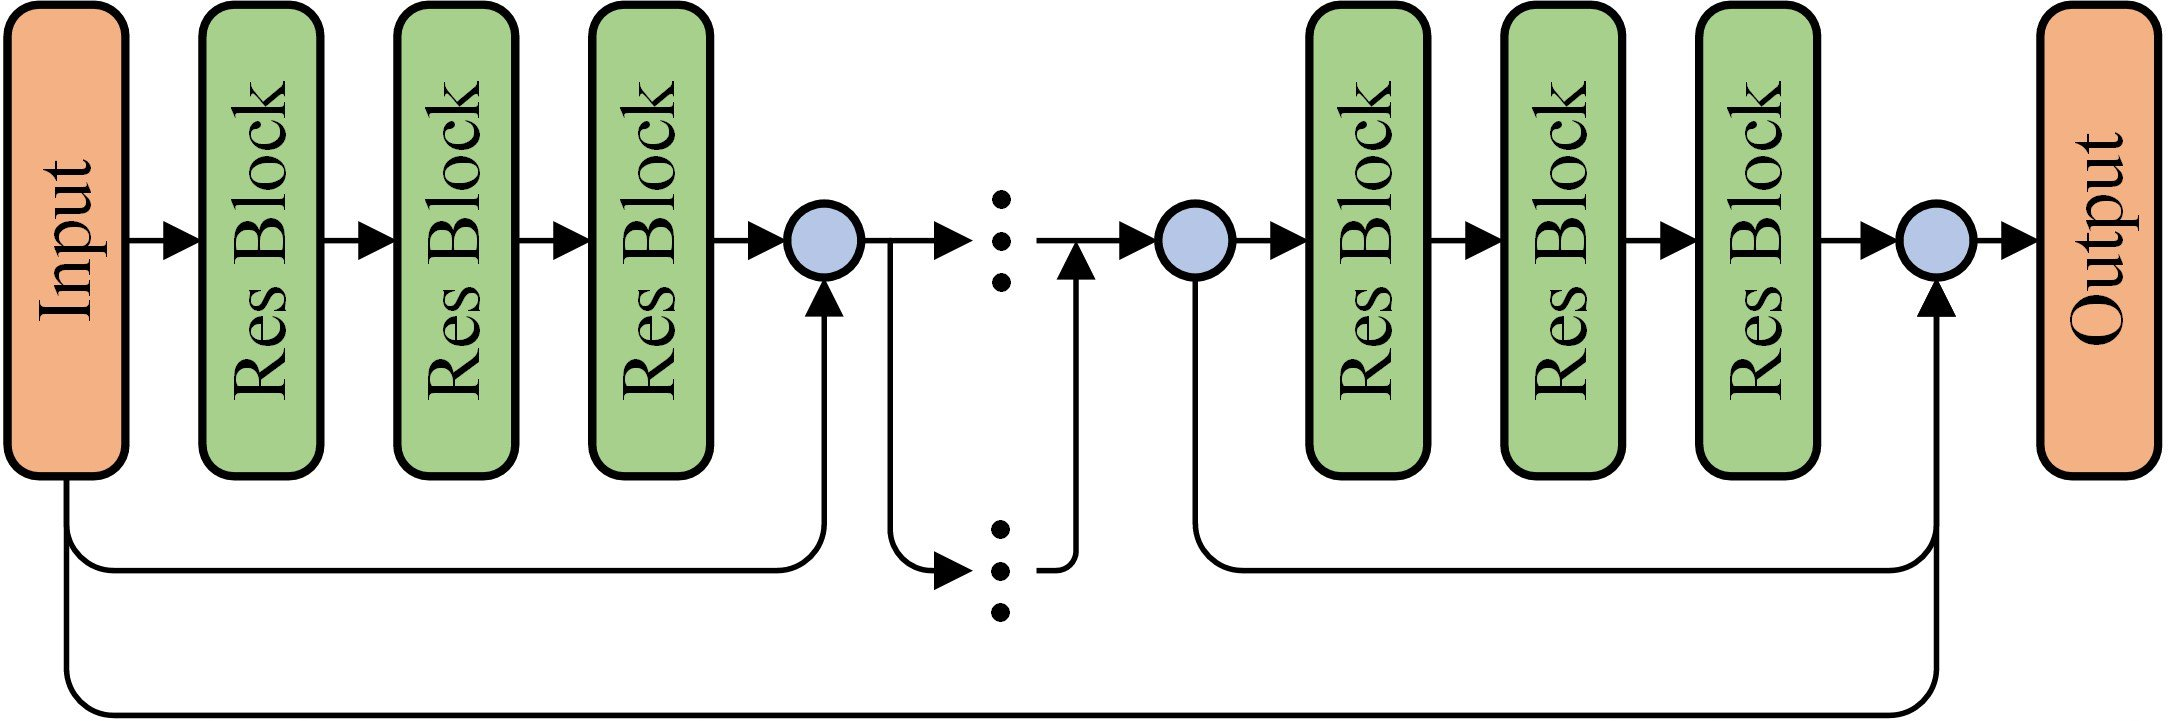
\includegraphics[width=0.9\columnwidth]{Imagens/An-illustration-of-the-deep-residual-network-ResNet-structure-More-shortcut.jpg}
    \caption{ Arquitetura de modelo base. Fonte:WikiCommons}
   \label{fig:ResNet-Rsp}
\end{figure}


\subsection{\textit{Treino}}\label{sec:Cap3_Treino}

Para a etapa de treino, utilizamos a arquitetura proposta em~\ref{sec:Cap3_Proposta}, que consiste em um modelo pré-treinado, e retreinando suas ultimas camadas de classificação por camadas fortemente conectadas seguidas de camadas de \textit{softmax}, como ilustra a imagem a seguir


\subsection{\textit{Validação}}\label{sec:Cap3_Validacao}

A etapa de validação será realizada a medida do desempenho do modelo no conjunto de testes para classificação.

\subsection{\textit{Seleção de modelos}}\label{sec:Cap3_SelecaoModelos}

Esta estapa concerne em gerar vários diferentes modelos e selecionar de acordo com a performance. É um processo experimental e de vasculhar diferentes hiperparâmetros e componentes do treino.



Critérios de seleção de modelo:
Melhor métrica f2 entre diferentes modelos. Com parada antecipada no menor valor de perda de validação em um treinamento, até no máximo à quinta época, devido a limitações de tempo e orçamento de horas de instâncias de GPU.
O segundo item foi possível de ser realizado. Realizando \textit{fine-tune} do modelo o modelo Resnet-16 inicialmente. Foram utilizados os pesos dessa mesma rede treinada para o dataset IMAGENET-1k, realizando a troca das camadas de saída, originalmente para 1000 classes. Foram Removidas e adicionados uma camada completamente conectada de entrada igual ao numero de neurônios da penultima camada. Após a ultima camada foi adicionado uma camada de sigmoid, que realizará a conversão de valores lineares para probabilidade de cada classe.

O modelo obteve um desempenho inicialmente satisfatório de métrica f2 de 0,88.

A partir deste modelo inicial, foram feitos vários ajustes de hiperparâmetros e de componentes a fim de aperfeiçoar o desempenho da rede. Dentre as os ajustes para seleção de modelo, constam:


\begin{enumerate}
    \item Pesos pré-treinados
    \item Aumentar capacidade da rede
    \item Adicionar regularização 
    \item Amostrador
    \item Aumento de dados aleatória
    \item Função de perda
    \item Otimizador
    \item Taxas de aprendizado
    \item Transferência de aprendizado vs Fine Tune
    \item Experimentar os mesmos passos para o modelo Swin-T
\end{enumerate}

Tendo inicialmente o modelo ResNet-18, os ajustes de capacidade de rede foram inicialmente se aumentar o número de camadas completamente conectadas, Contudo aumentar o número de camadas de blocos básicos resnet, utilizando o modelo ResNet50 demonstrou melhor métrica F2 e perda BCE. O mesmo foi testado utilizando com pesos do conjunto de dados ImageNet1k, igualmente com melhor resultados. Com pesos do trabalho~\ref{sec:Cap2_million} também de sensoriamento remoto, também ouve aumento expressivo de métrica F-2 em comparação com o modelo pre-treinado no conjunto de dados ImageNet-1k

Os modelos pré-treinados aparentavam convergir próximos da primeira época, o que sugere um rápido sobre-ajuste, para isto, testou-se utilizar um otimizador com decaimento de pesos o AdamW, porém leva a perda de performance, supostamente por afetar os pesos já treinados. O uso de regularização se limitou ao drop-out presente nos modelos e camadas de normalização de lote e camada.

Para mitigar o desbalanço de quantidade de amostras nas classes, investigou-se a utilização de outros amostradores, que escolhem amostras baseados em probabilidades especificadas pelo inverso da frequência de cada classe. Contudo não foi possível de ser realizado. O aumento de dados realizado foi aplicar espelho horizontal ou vertical com probabilidade de 25\%, dessa forma, o número de amostras é virtualmente aumentado para 4x o tamanho original.

Outra alternativa a mitigar o desbalanço foi alterar o valor da função de perda por classe, especificando que as classes mais raras realizariam um maior peso na função de perda. Esta alternativa gerou um aumento de performance, porém com rápido sobre-ajuste. Uma terceira alternativa foi a função de perda focal, que foi capaz de melhorar a métrica F2 substanciamente e mitigar sobreajuste da classe dominante.

Para o otimizador, há trabalhos como em\cite{https://doi.org/10.48550/arxiv.2106.10270}, que recomendam o uso de SGD para o ajuste-fino do modelo. Contudo apresentou convergência muito lenta, incompatível com o orçamento de horas de GPUs. O otimizador escolhido foi o Adam sem decaimento de peso. A convergência do modelo demonstrou-se sensível a taxa de aprendizado. Por isso, recorreu-se ao uso de taxas de aprendizado variáveis, utilizando um agendador de taxa de aprendizado, que reajusta para um décimo da anterior cada vez que a função de perda ou de métrica de validação atinge um platô.

Ainda na seleção de modelos, experimentou-se utilizar transferência de aprendizado, definida por congelar os pesos das camadas extratoras de características e treinar apenas ultimas camadas. Foi experimentado o ajuste fino, definido por retreinar o modelo inteiro, com as ultimas camadas inicializadas com pesos 0 ou aleatórios. A segunda opção demonstrou a melhor performance.


Os mesmos passsos foram realizados para o modelo Swin-T, chegando em uma iteração final de ambos modelos base e proposto.

\subsection{\textit{Treinamento Swin-T}}\label{sec:Cap3_TrainResnet}
Após a iteração final, foi registrado as métricas durante o treino no modelo restnet. Pelos gráficos 



\begin{figure}[!ht]
    \centering
    \includegraphics[width=\columnwidth]{Imagens/results/rsp-resnet-50_planet_pt/pontuação em treino e validação por época.jpg}
    \caption{ Arquitetura de modelo base.Fonte: Autor}
    \label{fig:TreinoResnetScore}
\end{figure}  

\begin{figure}[!ht]
    \centering
    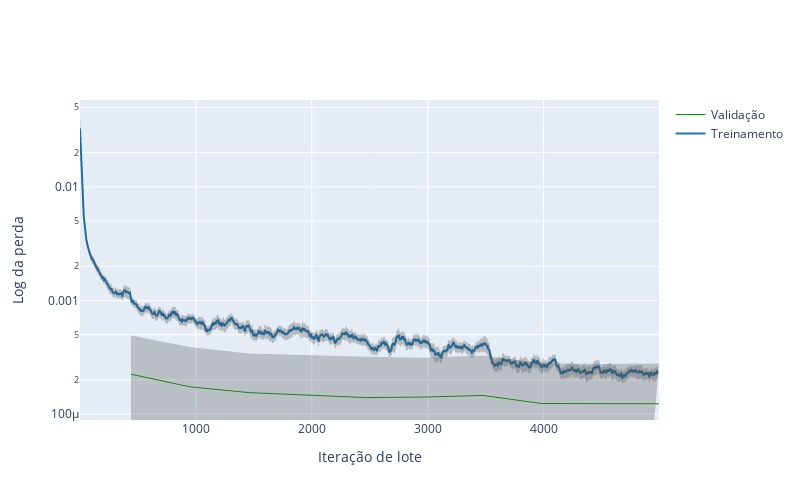
\includegraphics[width=\columnwidth]{Imagens/results/rsp-resnet-50_planet_pt/Training Loss Per Minibatch.jpg}
    \caption{ Arquitetura de modelo base. Fonte: Autor}
    \label{fig:TreinoResnetPerda}
\end{figure}


\subsection{\textit{Treinamento Swin-T}}\label{sec:Cap3_TrainSwinT}


\begin{figure}[!ht]
    \centering
    \includegraphics[width=\columnwidth]{Imagens/results/rsp-swin-t_planet_pt/pontuação em treino e validação por época.jpg}
    \caption{ Arquitetura de modelo base.Fonte: Autor}
    \label{fig:PontuacaoTrainSwin}
\end{figure}  

\begin{figure}[!ht]
    \centering
    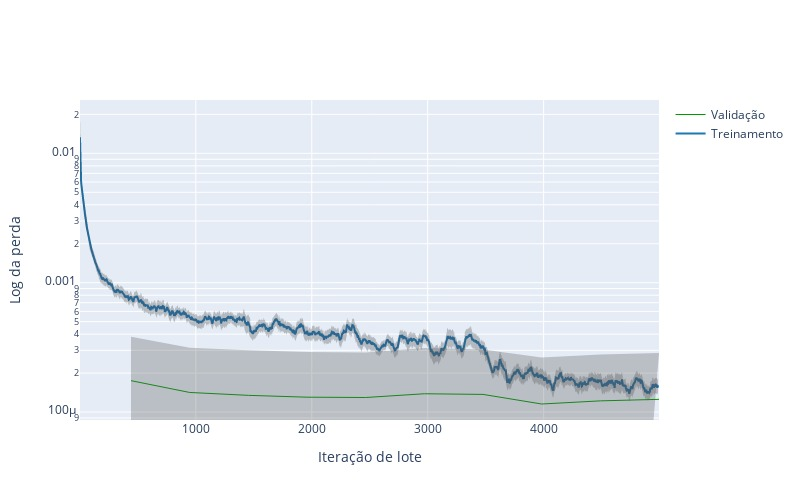
\includegraphics[width=\columnwidth]{Imagens/results/rsp-swin-t_planet_pt/Training Loss Per Minibatch.jpg}
    \caption{ Arquitetura de modelo base. Fonte: Autor}
    \label{fig:LossTrainSwin}
\end{figure}
